\documentclass{beamer}
\usepackage[T1]{fontenc}
\usepackage{latexsym,amsmath,amsthm,xcolor,multicol,booktabs,calligra,bookmark}
\usepackage{tikz,physics,subcaption}
\usepackage[compat=1.1.0]{tikz-feynman}
\usepackage{graphicx,pstricks,listings,stackengine}
\usepackage{hyperref}

\def\insertsupervisor{Prof. Giancarlo Ferrera}
\def\insertcosupervisor{Dr. Wan-Li Ju}

\author{JiaHao Miao}
\title{Resummation of QCD large infrared logarithms \\for Thrust distribution in \texorpdfstring{$e^+e^-$}{e+e-} annihilation}
\institute{
    Università degli Studi di Milano\\
    Dipartimento di Fisica "Aldo Pontremoli"
}

\date{\today}
\usepackage{style/Presentation}

% defs
\def\cmd#1{\texttt{\color{red}\footnotesize $\backslash$#1}}
\def\env#1{\texttt{\color{blue}\footnotesize #1}}
\definecolor{deepblue}{rgb}{0,0,0.5}
\definecolor{deepred}{rgb}{0.6,0,0}
\definecolor{deepgreen}{rgb}{0,0.5,0}
\definecolor{halfgray}{gray}{0.55}

\lstset{
    basicstyle=\ttfamily\small,
    keywordstyle=\bfseries\color{deepblue},
    emphstyle=\ttfamily\color{deepred},    % Custom highlighting style
    stringstyle=\color{deepgreen},
    numbers=left,
    numberstyle=\small\color{halfgray},
    rulesepcolor=\color{red!20!green!20!blue!20},
    frame=shadowbox,
}

\begin{document}

\begin{frame}
    \titlepage
\end{frame}

% Table of Contents slide
% \frame{\tableofcontents[sectionstyle=show,subsectionstyle=show/shaded/hide,subsubsectionstyle=show/shaded/hide]}

\section{Introduction}

\begin{frame}{Standard Model and QCD}
    \frametitle{The Standard Model of Particle Physics and QCD}
    \begin{columns}
        \begin{column}{0.5\textwidth}
            \scriptsize % or \footnotesize, \scriptsize, \tiny
            \textbf{Collider Physics:}
            \begin{itemize}
                \item Probing the fundamental structure of matter;
                \item Test of the Standard Model;
            \end{itemize}
            % \pause
            \textbf{The Standard Model:}
            \begin{itemize}
                \item A quantum field theory (QFT);
                \item Describes fundamental particles and interactions;
            \end{itemize}
            \begin{figure}[htpb]
                \centering
                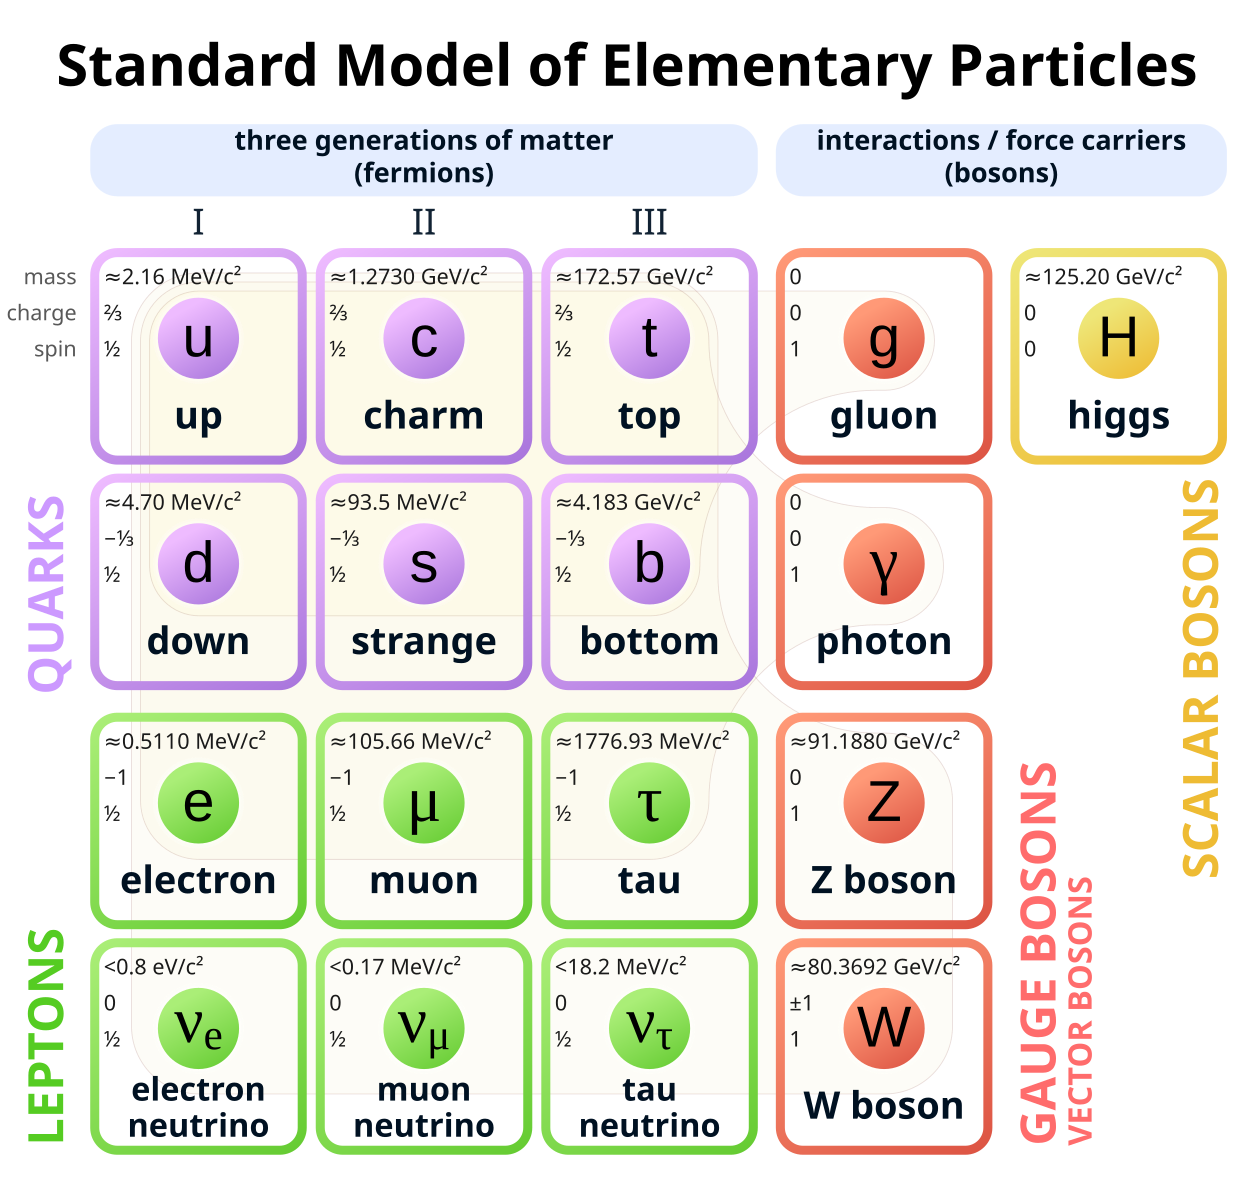
\includegraphics[width=0.7\textwidth]{figures/Standard_Model_of_Elementary_Particles.png}
            \end{figure}
        \end{column}
        % \pause
        \begin{column}{0.5\textwidth}
            \scriptsize
            \textbf{Quantum Chromodynamics (QCD):}
            \begin{itemize}
                \item Theory of the strong interaction;
                \item Running coupling constant $\alpha_s$;
                \item $\alpha_s(m_Z^2) = 0.1180 \pm  0.0009 $  \\
                (PDG 2023 average);
                \item Renormalization Group Equation\\
                $ \mu^2_R \frac{d \alpha_s}{d\mu^2_R} = - \alpha_s^2\sum_{i=0}^{\infty} b_{i} \alpha_s^{i}$;
                \item High energy $\to$ \alert{asymptotic freedom};
                \item Low energy $\to$ \alert{confinement};
                
            \end{itemize}
            \begin{figure}[h!]
                \centering
                
\includegraphics[width=\textwidth]{figures/alpha_running.png}
            \end{figure}
        \end{column}
    \end{columns}
\end{frame}

\section{Thrust distribution}

\begin{frame}{\textbf{Thrust: Definition}}
    \begin{equation*}
        T = \max_{\hat{n}} \frac{\sum_{i=1}^{N} | \vec{p}_i \cdot \hat{n} |}{\sum_{i=1}^{N} | \vec{p}_i |} = 1 - \tau
    \end{equation*} 
    \begin{itemize}
        \item $T$: Thrust
        \item $p_i$: Momentum of the $i$-th particle
        \item $\hat{n}$: Thrust axis, the direction that maximizes the thrust
        \item Infrared-safe observable: soft emission contribution drop out and collinear splitting doesn't affect the thrust value
        \item Thrust value ranges from 0.5 (isotropic) to 1 (pencil like)
    \end{itemize}
    
\end{frame}

\begin{frame}
    \begin{figure}
        \centering
        
\includegraphics[width=\textwidth]{figures/tau_maxVsN.png}
        \caption{The maximum value of thrust $\tau$ as a function of the number of partons $N$ in the final state.
        Optimization problem solved using Genetic Algorithm.}
    \end{figure}
\end{frame}

\begin{frame}
    \begin{figure}
        \centering
        
\includegraphics[width=0.9\textwidth]{figures/FOvsdata.png}
        \caption{Fixed Order calculations compared to experimental data.}
    \end{figure}
\end{frame}

\begin{frame}
    \begin{figure}
        \centering
        
\includegraphics[width=\textwidth]{figures/FO_tail_region_logplot.png}
        \caption{Log Plot of the Fixed Order calculations.}
    \end{figure}
\end{frame}

\begin{frame}{Thrust distribution}
    The Fixed Order expansion of the thrust distribution:
    \scriptsize
    \begin{align*}
        \frac{1}{\sigma_0} \dv{\sigma}{\tau} \qty(\tau,\mu) &= \delta(\tau) 
        + \overset{\alert{\text{LO}}}{\overbrace{\bar{\alpha}_s(\mu) \dv{A}{\tau}}}  
        + \overset{\alert{\text{NLO}}}{\overbrace{\bar{\alpha}_s^2(\mu) \dv{B}{\tau}}}  
        + \overset{\alert{\text{NNLO}}}{\overbrace{\bar{\alpha}_s^3(\mu) \dv{C}{\tau}}}
        + \order{\bar{\alpha}_s^4} , \\
        \dv{A}{\tau} \qty(\tau) &=  \frac{4}{3} \left(9 \tau -\frac{3}{\tau }+\left(-6 +\frac{4}{(1-\tau ) \tau }\right) \ln \left(\frac{1-2 \tau }{\tau }\right)+6\right),\\
        \frac{1}{\sigma_0}\dv{\sigma}{\tau} &\stackrel{\tau \to 0}{=} \delta(\tau) + \frac{2\alpha_s}{3\pi} \qty[\frac{-4 \ln \tau - 3}{\tau} + \dots]_{+} ,\\
        R_T(\tau) &= \int_0^\tau \frac{1}{\sigma_0}\dv{\sigma}{\tau'} \dd{\tau'} = 1 + \frac{2\alpha_s}{3\pi} \qty[-2 \ln^2 \frac{1}{\tau} + 3 \ln \frac{1}{\tau} + \dots].
    \end{align*}

    \normalsize
    \begin{itemize}
        \item $G_{nm} \bar{\alpha}_s^n \ln^m \frac{1}{\tau}$, with $m \le 2n $ plagues the fixed order expansion;
        \item \alert{Infrared Origin}: unbalanced cancellation of soft/collinear real and virtual contributions.
    \end{itemize}

\end{frame}

\section{Resummation of QCD large infrared logarithms}

\begin{frame}{Resummed distribution}
    \begin{figure}
        \centering
        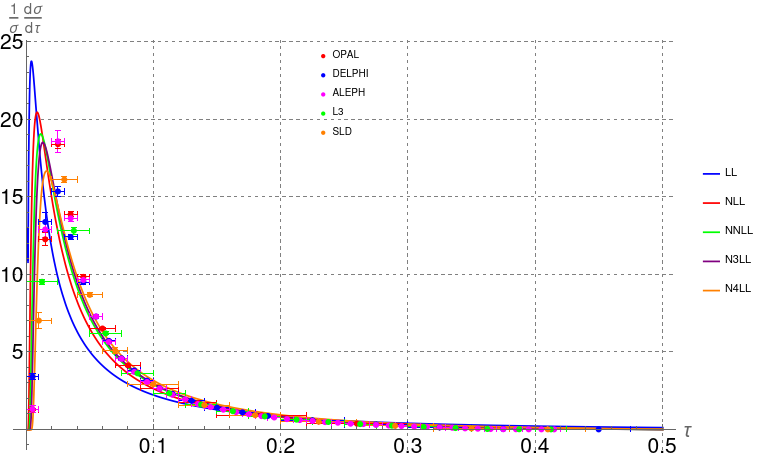
\includegraphics[width=0.8\textwidth]{figures/Thrust_differential_distribution_with_xerr.png}
        \caption{Resummed Distribution}
    \end{figure}
\end{frame}


\begin{frame}{Resummed distribution}
    \scriptsize
    \begin{align*}
        R_T(\tau,\mu) & \stackrel{\tau \to 0}{=} \qty(1 + \sum_{n=1}^{\infty} C_n \bar{\alpha}_s^n)\exp[L g_1(\lambda)  + \sum_{i=2} g_i(\lambda) \alpha_s^{i-2}]\\
        &= \qty(1 + \sum_{n=1}^{\infty} C_n \bar{\alpha}_s^n) \exp[\sum_{n=1}^\infty \bar{\alpha}_s^n \sum_{m=1}^{2n}G_{nm}\ln^m \frac{1}{\tau}]  ,\\
        &= 1 + R^{(1)}(\tau) \bar{\alpha}_s + R^{(2)}(\tau)\bar{\alpha}_s^2 + R^{(3)}(\tau)\bar{\alpha}_s^3+ \dots,\\
        R^{(n)}(\tau) &= \sum_{m=1}^{2n}R_{nm}\ln^m \frac{1}{\tau} + C_n  (\tau).
    \end{align*}
    
    \begin{table}[htpb]
        \centering
        \scriptsize
        \begin{tabular}{c c c c c c c }
            &&\(\text{LL}\) & \(\text{NLL}\) &\(\text{NNLL}\) & \(\text{N$^3$LL}\) & \(\text{N$^4$LL}\) \\
            \(\text{LO}\)&\(\bar{\alpha}_s^1\) &\(G_{12}\) & \(G_{11}\) & \(C_1\) & -  & -  \\
            \(\text{NLO}\)&\(\bar{\alpha}_s^2\) & \(G_{23}\) & \(G_{22}\) & \(G_{21}\) & \(C_2\) & - \\
            \(\text{NNLO}\)&\(\bar{\alpha}_s^3\) & \(G_{34}\) & \(G_{33}\) & \(G_{32}\) & \(G_{31}\) & \(C_3\)\\
            \(\text{N$^3$LO}\)&\(\bar{\alpha}_s^4\) & \(G_{45}\) & \(G_{44}\) & \(G_{43}\) & \(G_{42}\) & \(G_{41}\) \\
        \end{tabular}
    \end{table}
    
\end{frame}

\begin{frame}{Resummed distribution LogPlot}
    \begin{figure}
        \centering
        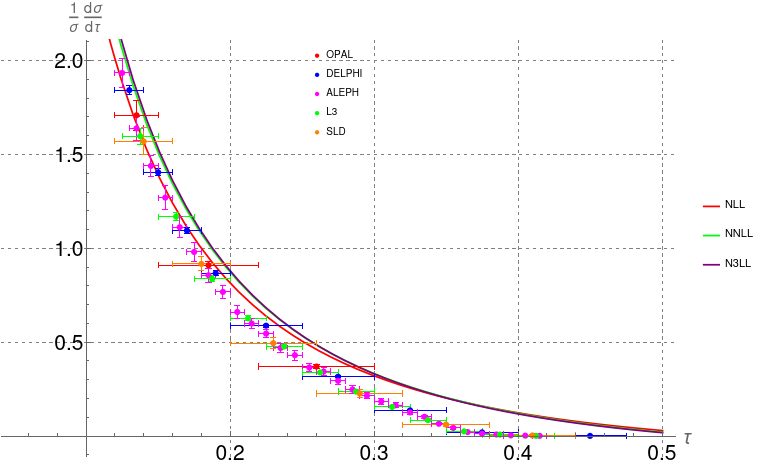
\includegraphics[width=0.8\textwidth]{figures/Resummed_tail_region.png}
        \caption{Resummed Distribution LogPlot}
    \end{figure}
\end{frame}

\begin{frame}{Matched distribution}
    \scriptsize
    \begin{align*}
        R_T(\tau,\mu) &= \qty(1 + \sum_{n=1}^{\infty} C_n \bar{\alpha}_s^n)\exp[L g_1(\lambda)  + \sum_{i=2} g_i(\lambda) \alpha_s^{i-2}] \alert{+ D\qty(\tau,\alpha_s\qty(Q^2))}\\
        &= \qty(1 + \sum_{n=1}^{\infty} C_n \bar{\alpha}_s^n) \exp[\sum_{n=1}^\infty \bar{\alpha}_s^n \sum_{m=1}^{2n}G_{nm}\ln^m \frac{1}{\tau}] \alert{+ D\qty(\tau,\alpha_s\qty(Q^2))} ,\\
        &= 1 + R^{(1)}(\tau) \bar{\alpha}_s + R^{(2)}(\tau)\bar{\alpha}_s^2 + R^{(3)}(\tau)\bar{\alpha}_s^3+ \dots \alert{+ D\qty(\tau,\alpha_s\qty(Q^2))},\\
        R^{(n)}(\tau) &= \sum_{m=1}^{2n}R_{nm}\ln^m \frac{1}{\tau} + C_n \\
        D_1(\tau) &=  A(\tau) - R^{(1)}(\tau),\\
        D_2(\tau) &=  B(\tau) - R^{(2)}(\tau),\\
        D_3(\tau) &=  C(\tau) - R^{(3)}(\tau).
    \end{align*}
    
    % \begin{table}[htpb]
    %     \centering
    %     \scriptsize
    %     \begin{tabular}{c c c c c c c }
    %         &&\(\text{LL}\) & \(\text{NLL}\) &\(\text{NNLL}\) & \(\text{N$^3$LL}\) & \(\text{N$^4$LL}\) \\
    %         \(\text{LO}\)&\(\bar{\alpha}_s^1\) &\(R_{12}\) & \(R_{11}\) & \(C_1+D_1(\tau)\) & -  & -  \\
    %         \(\text{NLO}\)&\(\bar{\alpha}_s^2\) & \(R_{23}\) & \(R_{22}\) & \(R_{21}\) & \(C_2 + D_2(\tau)\) & - \\
    %         \(\text{NNLO}\)&\(\bar{\alpha}_s^3\) & \(R_{34}\) & \(R_{33}\) & \(R_{32}\) & \(R_{31}\) & \(C_3 + D_3(\tau)\)\\
    %         \(\text{N$^3$LO}\)&\(\bar{\alpha}_s^4\) & \(R_{45}\) & \(R_{44}\) & \(R_{43}\) & \(R_{42}\) & \(R_{41}\) \\
    %     \end{tabular}
    % \end{table}
    
\end{frame}

\begin{frame}{Matched distribution}
    \begin{figure}
        \centering
        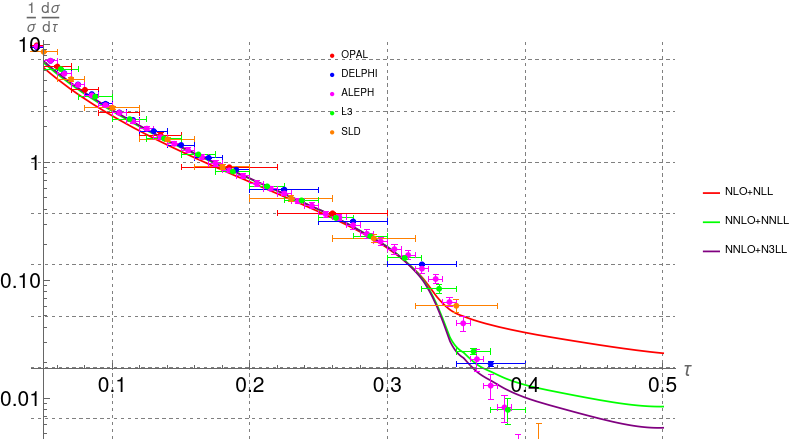
\includegraphics[width=0.8\textwidth]{figures/matched_tail_region_logplot.png}
        \caption{Matched Distribution LogPlot}
    \end{figure}
\end{frame}

\begin{frame}{Matched distribution}
    \begin{figure}
        \centering
        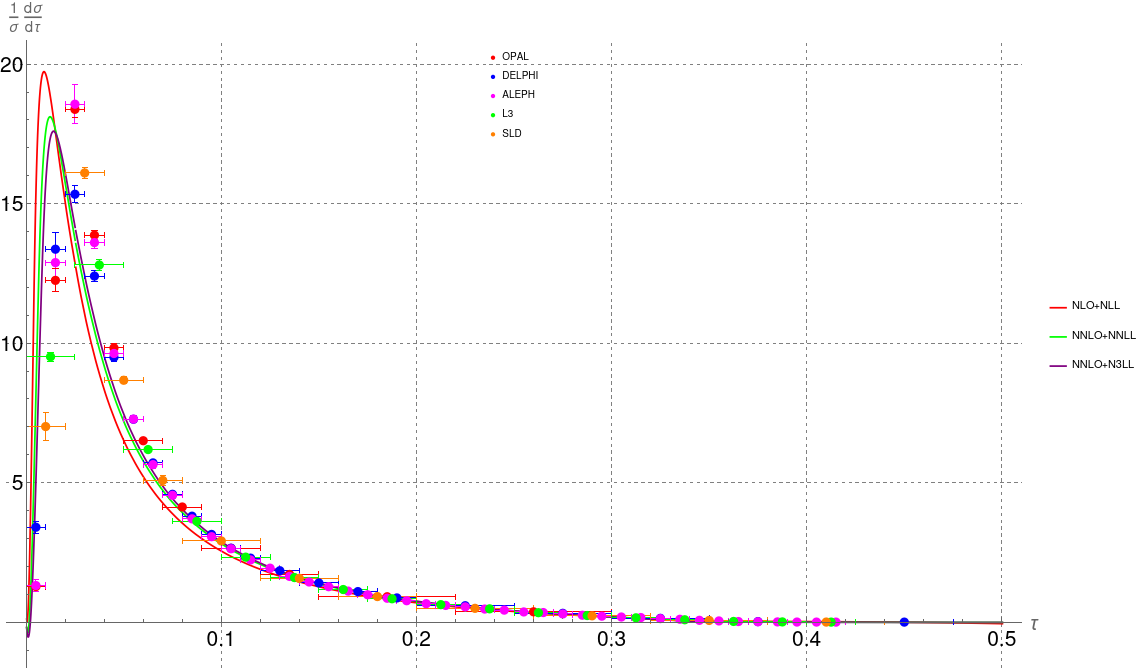
\includegraphics[width=0.8\textwidth]{figures/Matching.png}
        \caption{Matched Distribution}
    \end{figure}
\end{frame}

\begin{frame}{Preliminary Results}
    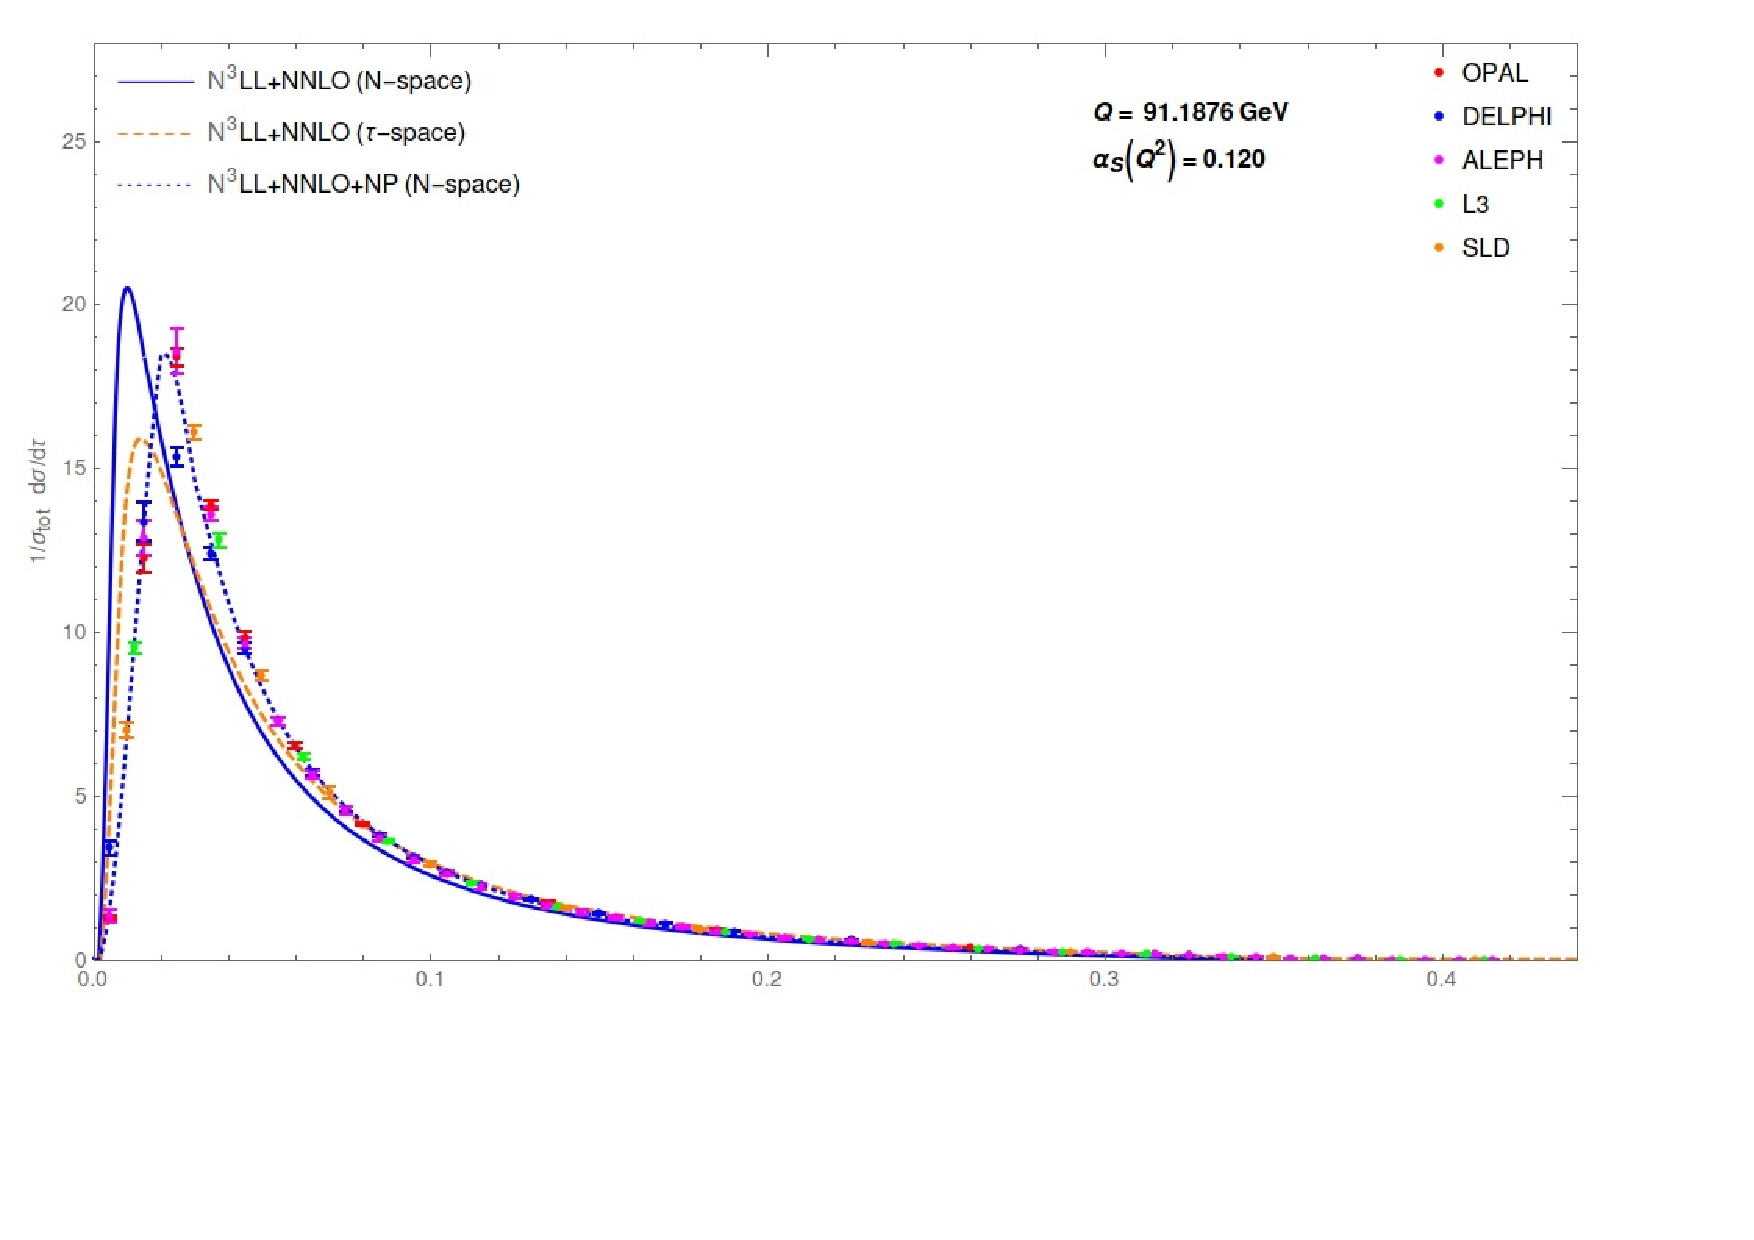
\includegraphics[width=0.95\linewidth]{figures/thrust-resNP2.pdf}
\end{frame}


\section{Conclusion}

% \begin{frame}{Conclusion}
%     In this work:
%     \begin{itemize}
%         \item Calculated resummation functions \( f_i(\lambda) \) in Laplace space, ensuring consistency and extending to N$^4$LL accuracy;
%         \item Performed inverse Laplace transform for resummed distribution;
%         \item Matched resummed expression to NNLO fixed-order calculations using the R-matching scheme;
%         \item Achieved NNLO+N$^3$LL accuracy for Thrust distribution predictions.
%     \end{itemize}
% \end{frame}

\begin{frame}{Summary and Future Work}
    \scriptsize
    In this work I have:
    \begin{itemize}
        \item Calculated resummation functions \( f_i(\lambda) \) in Laplace space, ensuring consistency and extending to N$^4$LL accuracy;
        \item Performed inverse Laplace transform for resummed distribution;
        \item Matched resummed expression to NNLO fixed-order calculations using the R-matching scheme;
        \item Achieved NNLO+N$^3$LL accuracy for Thrust distribution predictions.
    \end{itemize}
    
    Future developments:
    \begin{itemize}
        \item Integrate phenomenological model for hadronization effects;
        \item Conduct fitting analysis with experimental data for accurate \( \alpha_s \) determination;
        \item Investigate reliability of analytical Laplace inversion for higher orders;
        \item Address discrepancies in peaks of resummed Thrust distribution compared to experimental data.
    \end{itemize}
\end{frame}

\begin{frame}
    \begin{center}
        {\Huge\calligra Thank You!}
    \end{center}
\end{frame}

% Backup Slides
\appendix
\backupbegin

\begin{frame}
    \scriptsize
    \begin{columns}
        \begin{column}{0.5\textwidth}
            \begin{figure}
                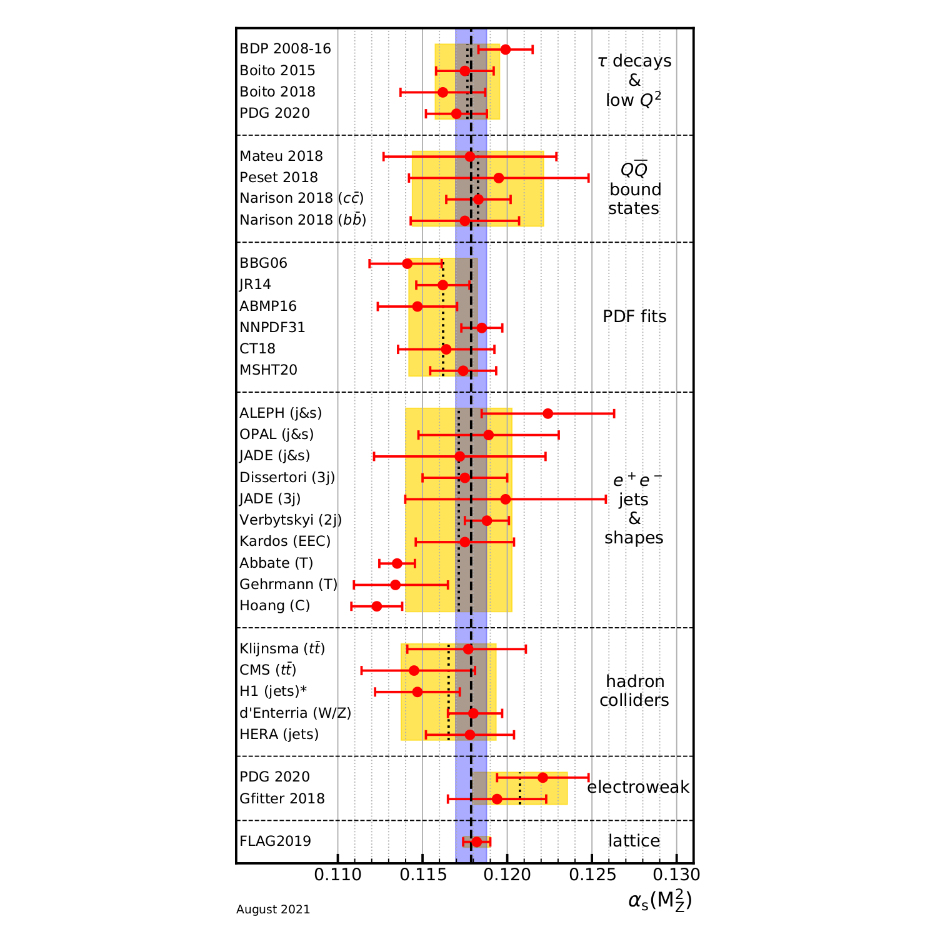
\includegraphics[scale=0.2]{figures/pdg2021.png}
                \caption{Particle Data Group 2021 average of $\alpha_s$}
            \end{figure}
        \end{column}
        \begin{column}{0.5\textwidth}
            \begin{figure}
                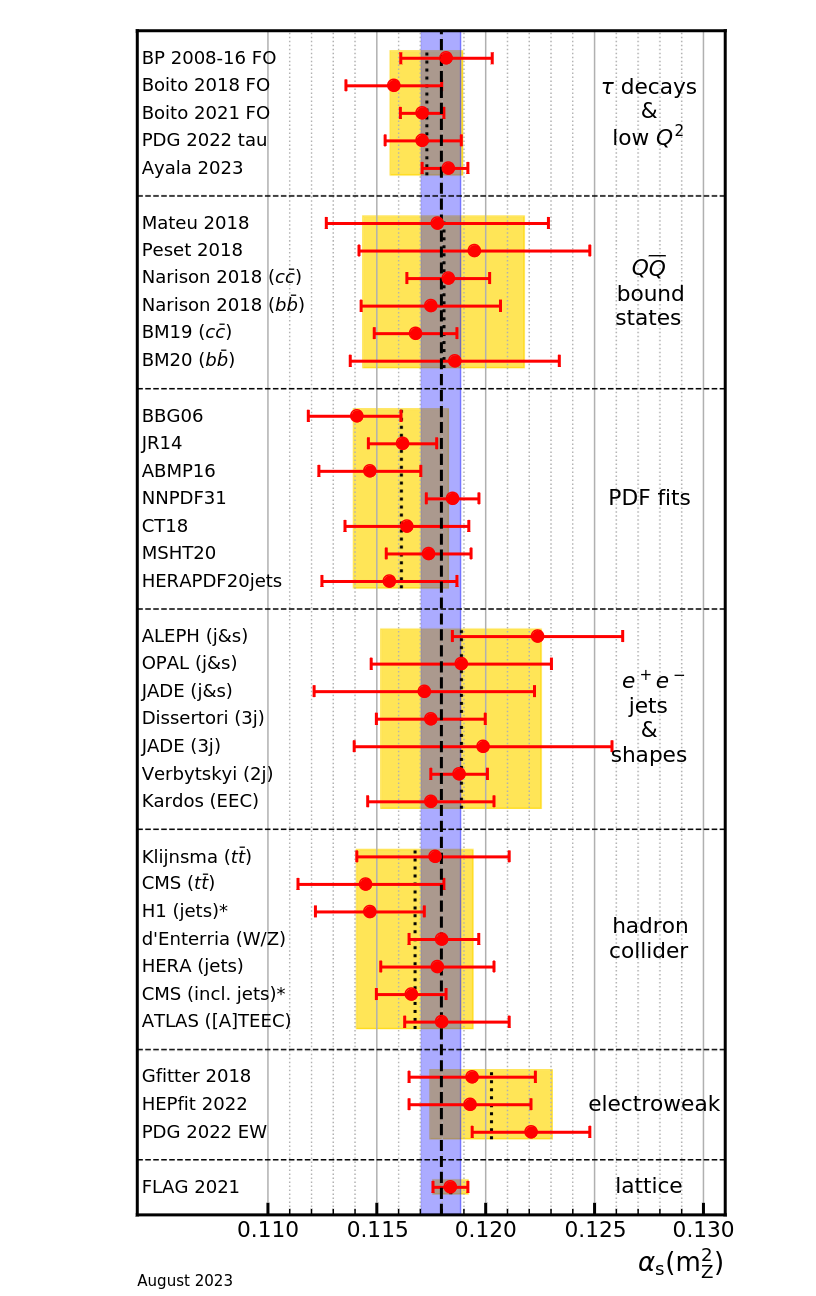
\includegraphics[scale=0.15]{figures/pdg2023.png}
                \caption{Particle Data Group 2023 average of $\alpha_s$}
            \end{figure}
        \end{column}
    \end{columns}
\end{frame}

\begin{frame}{How to find the Thrust axis}
    \scriptsize
    Given a set of $N$ partons in the final state with momenta $\vec{p}_i$, the optimization problem for the thrust 
    can be reduced to a combinatorial problem:

    \begin{align*}
        \vec{p}_j\cdot \vec{n} &= s_j \vert \vec{p}_j\cdot \vec{n} \vert \qq{with $s_j = \pm 1$},\\
        T &= \max_{\vec{n}} \frac{\sum_j \vert \vec{p}_j\cdot \vec{n} \vert}{\sum_j \vert \vec{p}_j \vert} = \max_{\vec{n}} \frac{\sum_j s_j \vec{p}_j\cdot \vec{n}}{\sum_j \vert \vec{p}_j \vert} = \max_{\vec{n}} \frac{\vec{P}\cdot \vec{n}}{\sum_i \vert \vec{p}_i \vert} \\
        \vec{P} &= \sum_j s_j \vec{p}_j.
    \end{align*}
    
    \begin{itemize}
        \item $2^N$ possible configurations for the $s_j$;
        \item Thrust invariant under $\vec{n} \to -\vec{n}$ transformation, $\to$ $2^{N-1}$ configurations;
        \item The configuration of all 1's and -1's doesn't respect the momentum conservation, $\to$ $2^{N-1}-1$ configurations to check; 
        \item Check the $2^{N-1}-1$ configurations to find $\vec{P}$
        \item Thrust axis is $\vec{n}= \frac{\vec{P}}{|\vec{P}|}$
    \end{itemize}

\end{frame}


\begin{frame}
    \begin{figure}
        \centering
        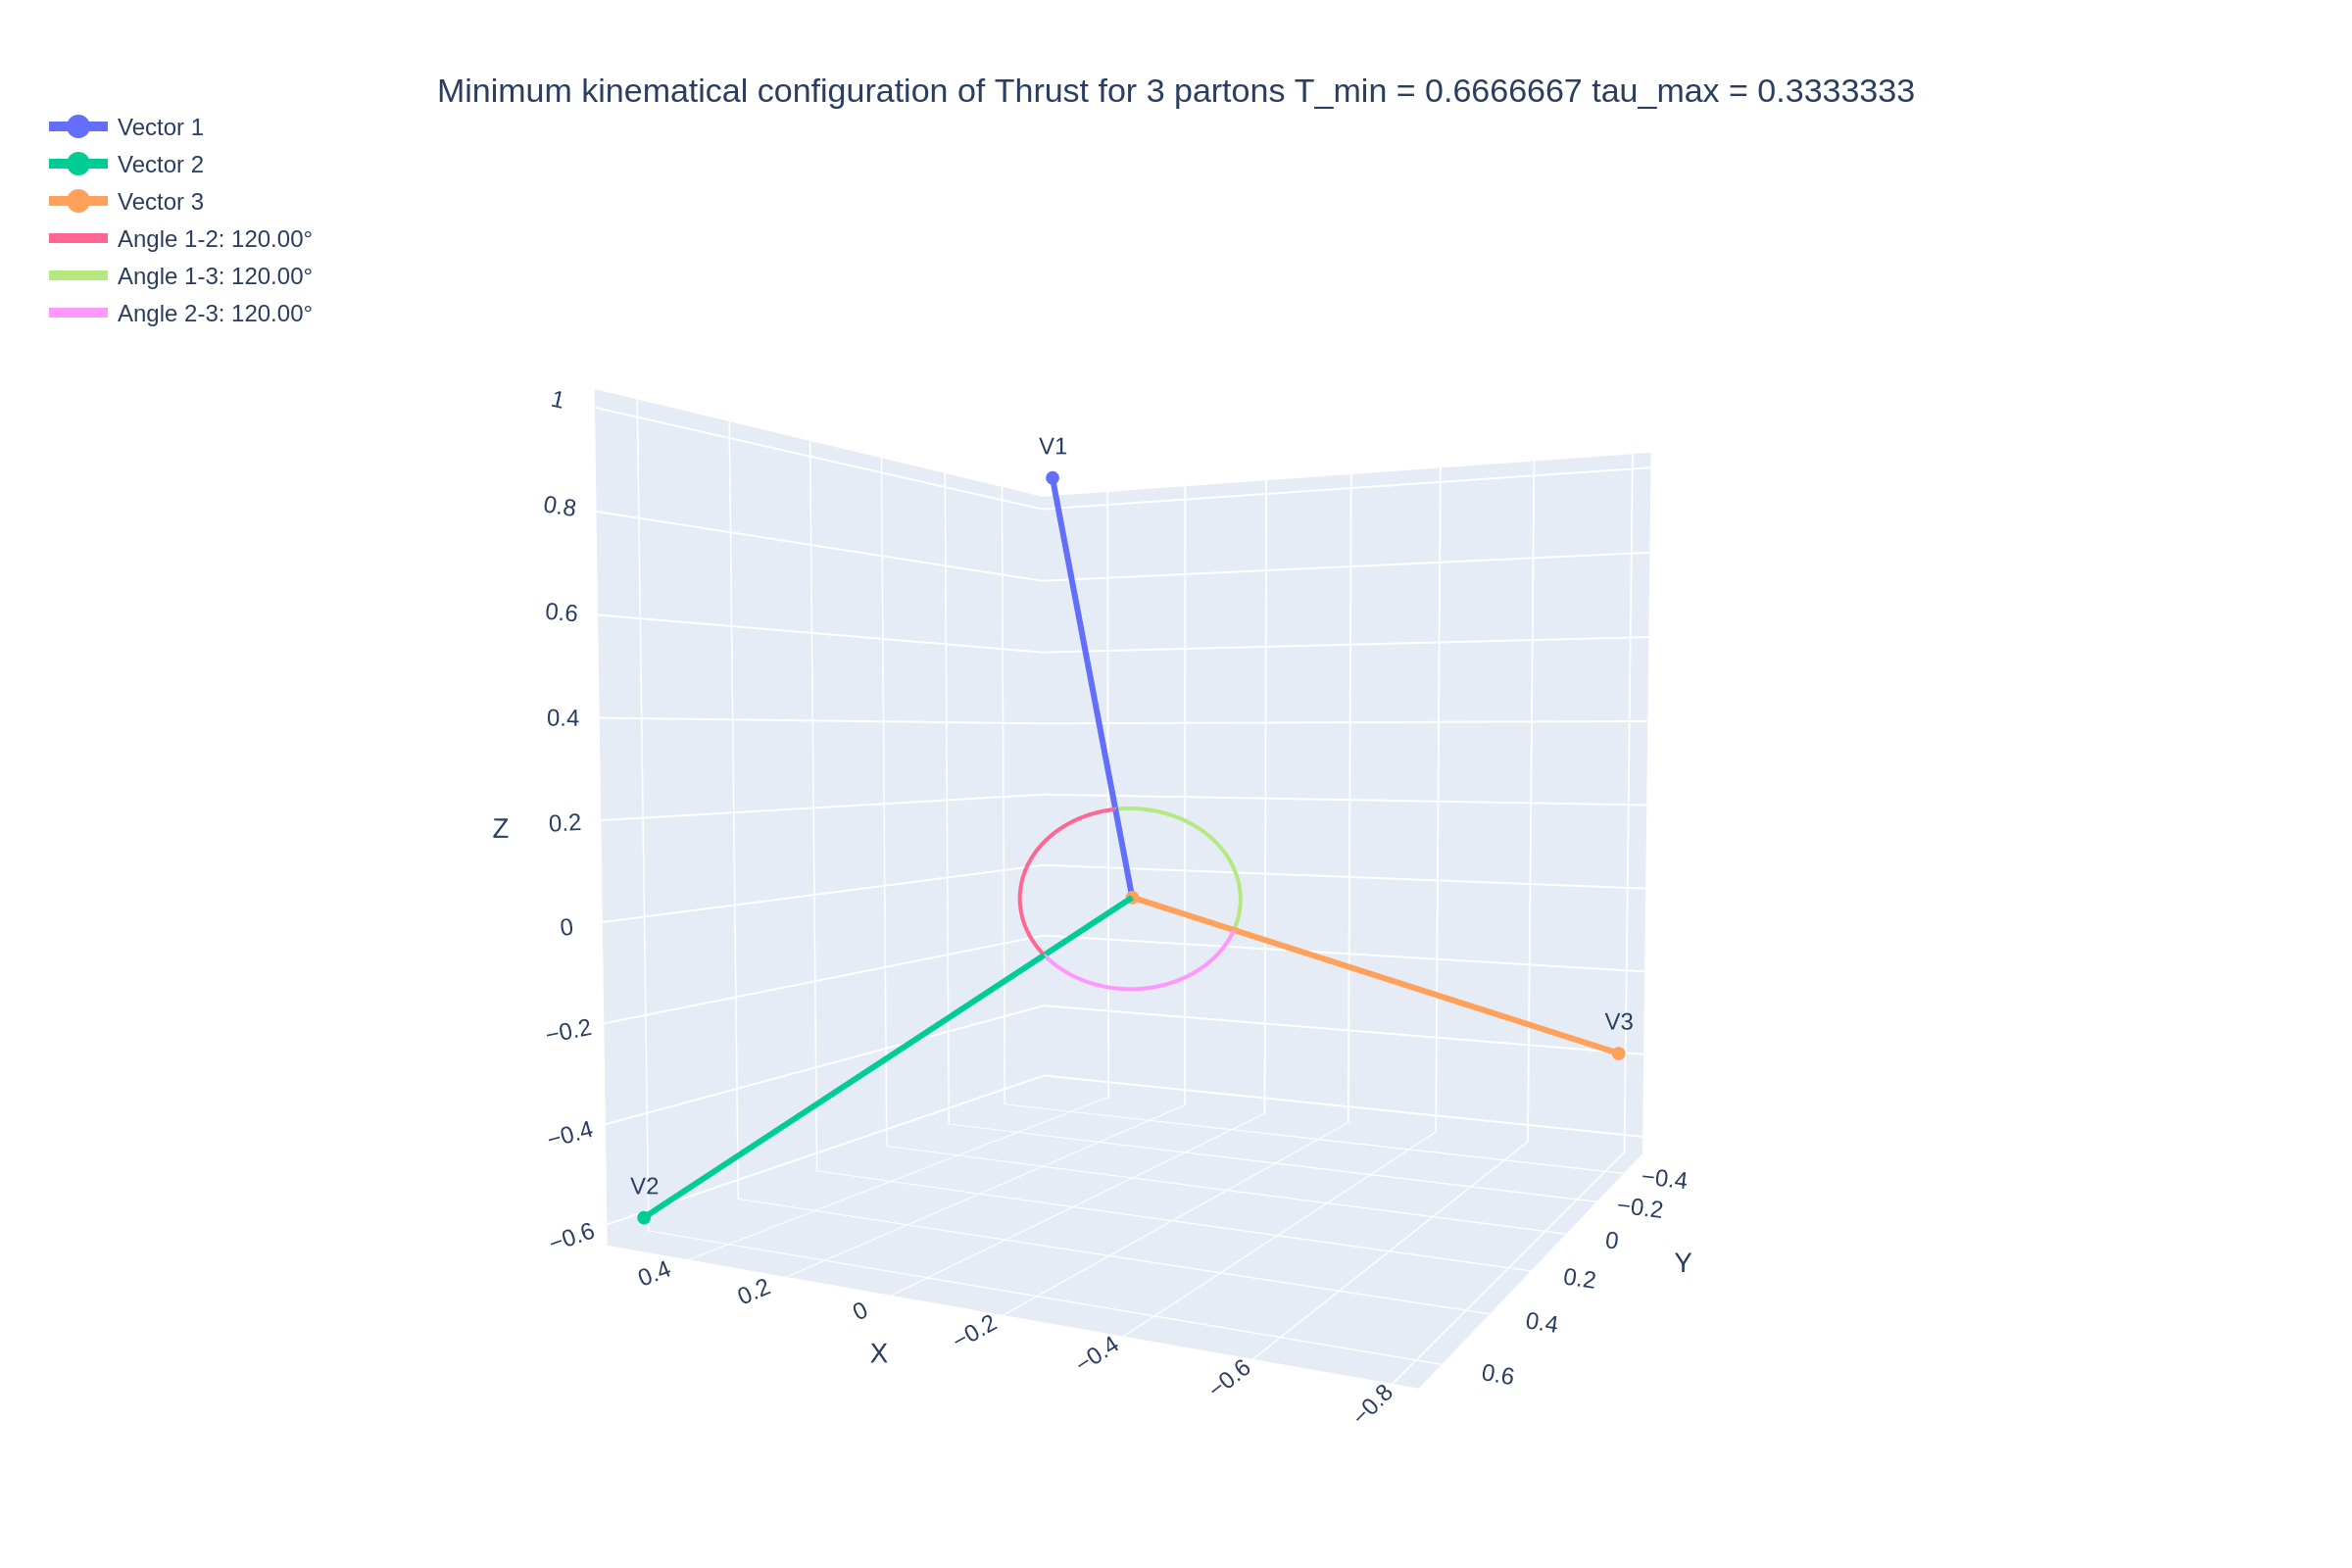
\includegraphics[width=0.8\textwidth]{figures/plot_3_partons.png}
        \caption{Kinematic configuration of the three partons in the final state that minimizes the thrust.}
    \end{figure}
\end{frame}

\begin{frame}
    \begin{figure}
        \centering
        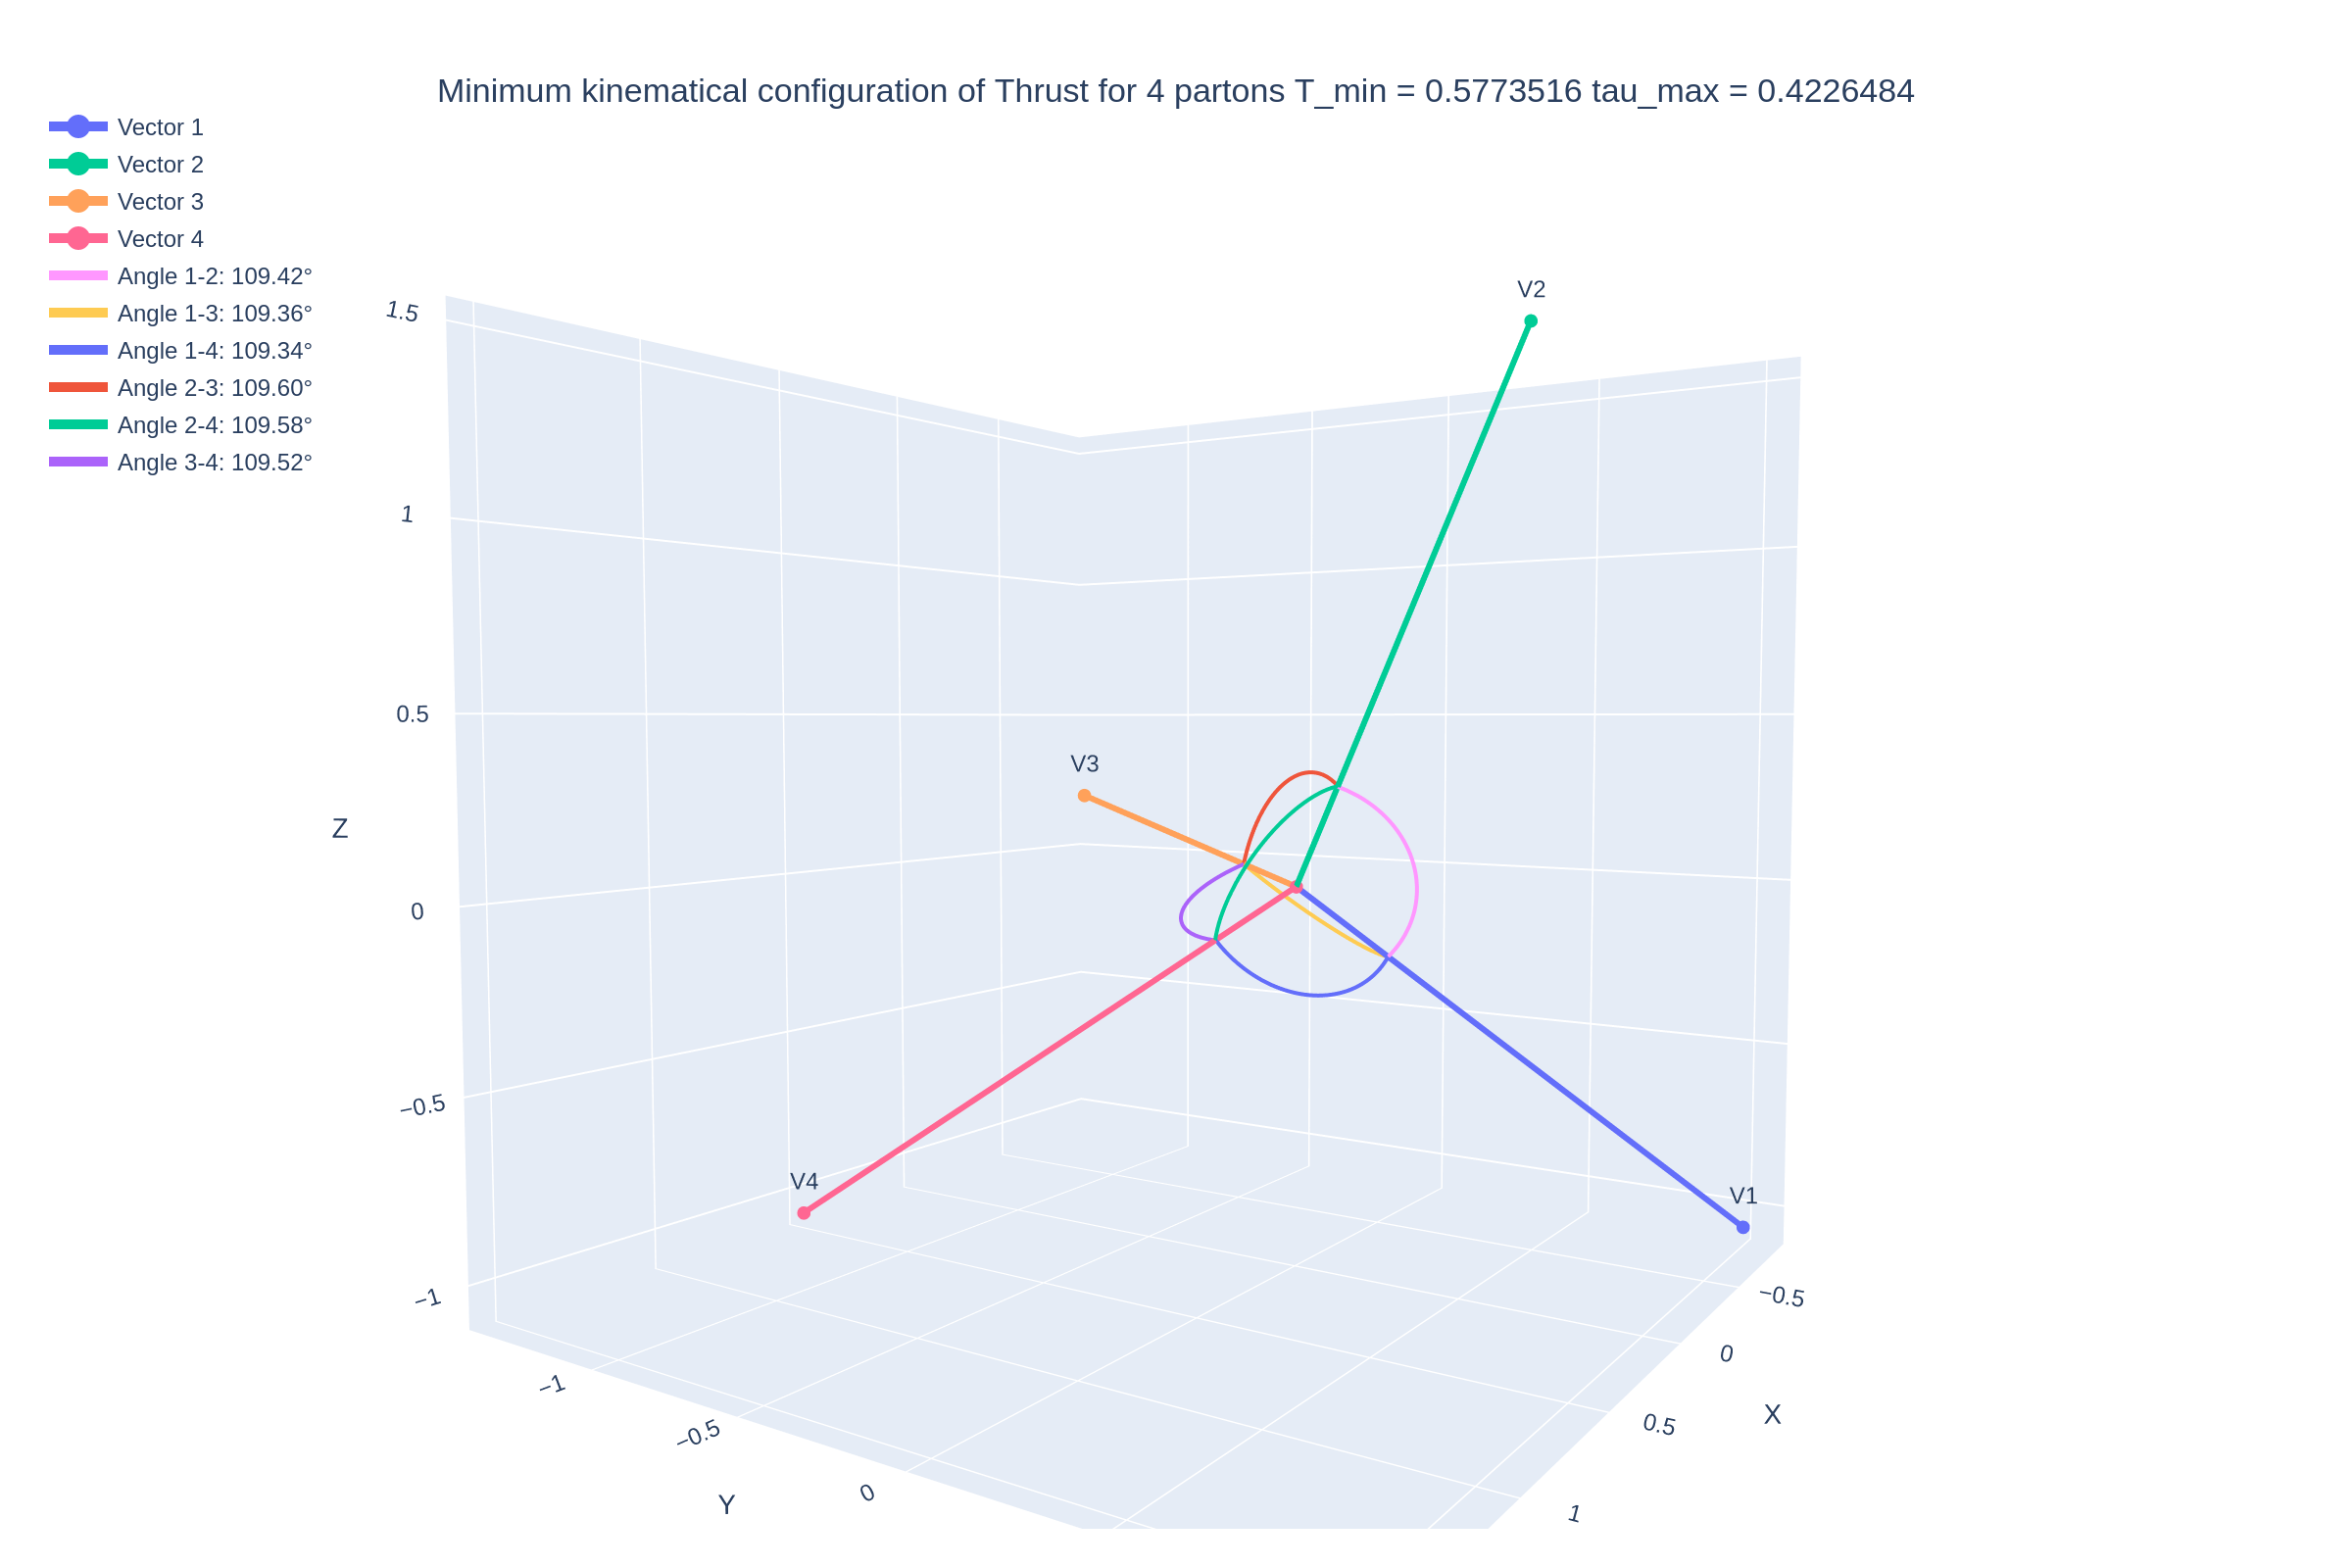
\includegraphics[width=0.8\textwidth]{figures/plot_4_partons.png}
        \caption{Kinematic configuration of the four partons in the final state that minimizes the thrust.}
    \end{figure}
\end{frame}

\begin{frame}
    \begin{figure}
        \centering
        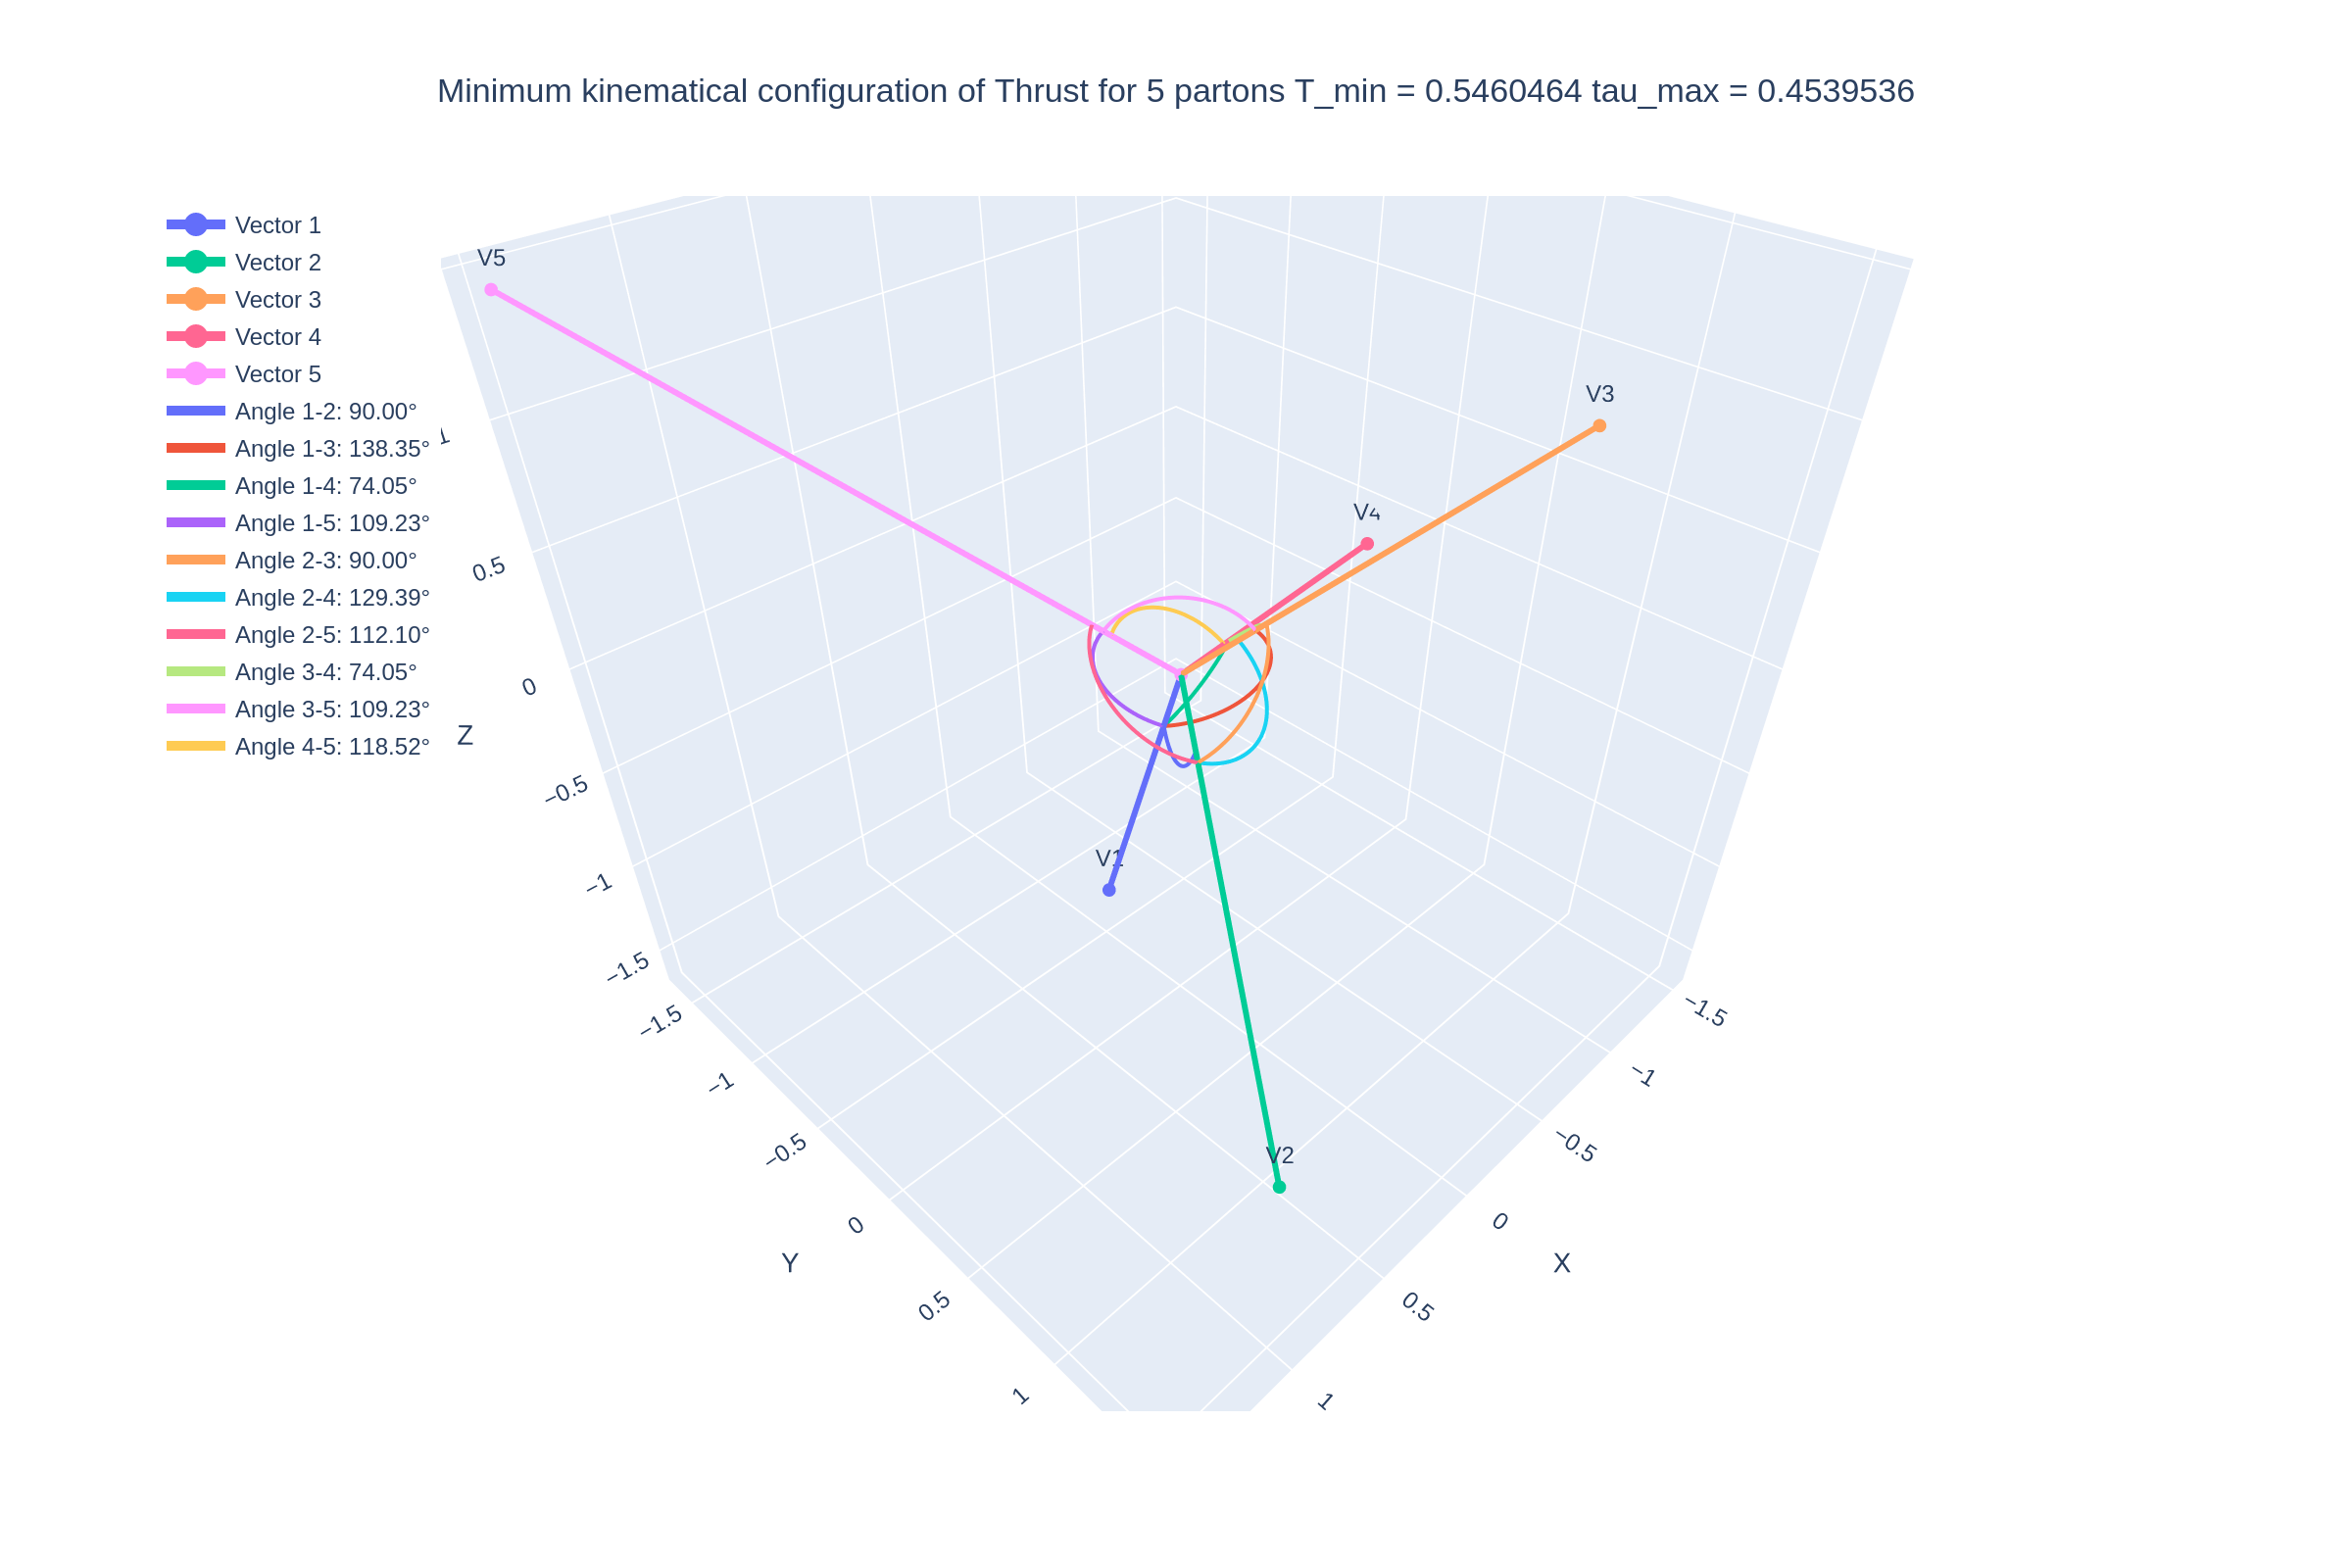
\includegraphics[width=0.9\textwidth]{figures/plot_5_partons.png}
        \caption{Approximate Kinematic configuration of the five partons in the final state that minimizes the thrust.}
    \end{figure}
\end{frame}

\begin{frame}{Real and Virtual Contributions}
    \begin{itemize}
        \item \alert{Infrared Origin}: unbalanced cancellation of soft/collinear real and virtual contributions.
    \end{itemize}
    
    \centering
    \resizebox{\linewidth}{!}{%
        \begin{tikzpicture}
            % First Feynman diagram
            \node at (0,0) {
                \begin{tikzpicture}
                    \begin{feynman}
                        \vertex (a);
                        \vertex [above left=of a] (i1) {$e^{-}$};
                        \vertex [below left=of a] (i2) {$e^{+}$};
                        \vertex (b) [right=of a];
                        \vertex [above right=of b] (f1) {$q$};
                        \vertex [below right=of b] (f2) {$\bar{q}$};
        
                        \diagram* {
                            (i1) -- [fermion] (a) -- [fermion] (i2),
                            (a) -- [photon, edge label=\(\gamma^* / Z\), momentum'=\(k\)] (b),
                            (f2) -- [fermion] (b) -- [fermion] (f1),
                        };
                    \end{feynman}
                \end{tikzpicture}
            };
            % Second Feynman diagram
            \node at (5,0) {
                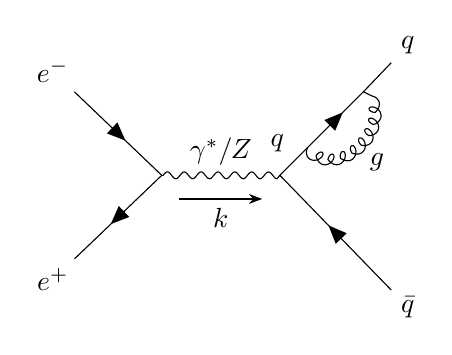
\begin{tikzpicture}
                    \begin{feynman}
                        \vertex (a);
                        \vertex [above left=of a] (i1) {$e^{-}$};
                        \vertex [below left=of a] (i2) {$e^{+}$};
                        \vertex (b) [right=of a];
                        \vertex [above right=0.5cm of b] (f1);
                        \vertex (c) [above right=0.5cm of b];
                        \vertex (d) [above right=1cm of c];
                        \vertex [above right=0.5cm of d] (f3) {$q$};
                        \vertex [below right=2cm of b] (f2) {$\bar{q}$};
        
                        \diagram* {
                            (i1) -- [fermion] (a) -- [fermion] (i2),
                            (a) -- [photon, edge label=\(\gamma^* / Z\), momentum'=\(k\)] (b),
                            (f2) -- [fermion] (b) -- [edge label=\(q\)] (f1),
                            (c) -- [gluon, edge label'=$g$, half right] (d),
                            (c) -- [fermion] (d),
                            (d)-- (f3),
                        };
                    \end{feynman}
                \end{tikzpicture}
            };
            % Third Feynman diagram
            \node at (10,0) {
                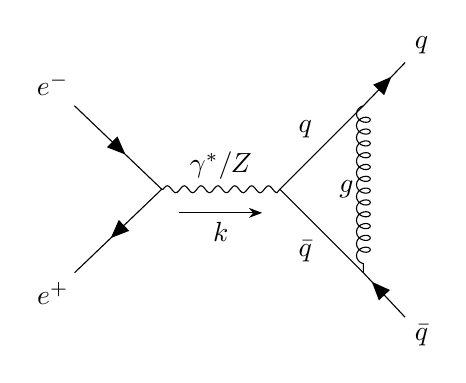
\begin{tikzpicture}
                    \begin{feynman}
                        \vertex (a);
                        \vertex [above left=of a] (i1) {$e^{-}$};
                        \vertex [below left=of a] (i2) {$e^{+}$};
                        \vertex (b) [right=of a];
                        \vertex [above right=of b] (c);
                        \vertex [below right=of b] (d);
                        \vertex [above right=0.75cm of c] (f1) {$q$};
                        \vertex [below right=0.75cm of d] (f2) {$\bar{q}$};
        
                        \diagram* {
                            (i1) -- [fermion] (a) -- [fermion] (i2),
                            (a) -- [photon, edge label=\(\gamma^* / Z\), momentum'=\(k\)] (b),
                            (d) -- [edge label=\(\bar{q}\)] (b) -- [edge label=\(q\)] (c),
                            (c) -- [gluon, edge label'=$g$] (d),
                            (c) -- [fermion] (f1),
                            (d) -- [anti fermion] (f2),
                        };
                    \end{feynman}
                \end{tikzpicture}
            };
        \end{tikzpicture}
    }
\end{frame}

\begin{frame}{Infrared-safety}

    \begin{equation*}
        T = \max_{\hat{n}} \frac{\sum_{i=1}^{N} | \vec{p}_i \cdot \hat{n} |}{\sum_{i=1}^{N} | \vec{p}_i |} = 1 - \tau
    \end{equation*} 
    
    \begin{itemize}
        \item Infrared-safe observable: soft emission contribution drop out and collinear splitting doesn't affect the thrust value
    \end{itemize}

    \begin{flalign*}
        &\vert (1-\lambda)\vec{p_i}\cdot \vec{n} \vert + \vert \lambda \vec{p_i}\cdot \vec{n}\vert =(1-\lambda)\vert\vec{p_i}\cdot \vec{n} \vert + \lambda \vert \vec{p_i}\cdot \vec{n}\vert = \vert \vec{p_i}\cdot \vec{n} \vert ,\\
        &\vert (1-\lambda)\vec{p_i} \vert + \vert \lambda \vec{p_i}\vert = (1-\lambda) \vert \vec{p_i} \vert + \lambda \vert\vec{p_i}\vert = \vert \vec{p_i} \vert .
    \end{flalign*}
    
\end{frame}

\begin{frame}{Calculations}
    \scriptsize
    \begin{align*}
        \ln \Tilde{J}_\nu^q(Q^2) &= - \int_{N_0/N}^{1} \frac{\dd u}{u} \qty[ \int_{u^2 Q^2}^{u Q^2} \frac{1}{q^2} A\qty(\alpha_s(q^2)) \dd q^2 + \frac{1}{2} B \qty(\alpha_s(u Q^2))]\\
        &+ \ln \Tilde{C}\qty(\alpha_s(\mu^2),\frac{\mu^2}{Q^2}),\\
        A(\alpha_s) &= \sum_{n=1}^\infty A_n \qty(\frac{\alpha_s}{\pi})^n, \\
        B(\alpha_s) &= \sum_{n=1}^\infty B_n\qty(\frac{\alpha_s}{\pi})^n,\\
        \ln \Tilde{J}_\nu^q(Q^2) &= \ln N f_1(\lambda) + f_2(\lambda) + \alpha_s f_3(\lambda) + \alpha_s^2 f_4(\lambda) + \alpha_s^3 f_5(\lambda) + \order{\alpha_s^n \ln^{n-4}N} \nonumber\\
        &+ \ln \Tilde{C}\qty(\alpha_s(\mu^2),\frac{\mu^2}{Q^2}).
    \end{align*}
\end{frame}

\begin{frame}{Inverse Laplace Transform}
    \scriptsize
    \begin{align*}
        J^q(Q^2,k^2) &= \frac{1}{2\pi i} \lim_{T \to \infty}\int_{C-iT}^{C+iT} \dd \nu e^{\nu k^2} \tilde{J}^q_\nu \qty(Q^2),\\
        R^q(w) &= \frac{1}{2\pi i} \int_C \frac{\dd u}{u} e^{u} e^{\mathcal{F}(\alpha_s,\ln u + L)} \\
        &\stackrel{\text{Taylor}}{=} \int_C \frac{\dd u}{2\pi i} e^{u-\ln u} e^{\mathcal{F}(\alpha_s,L)+\sum_{n=1}^\infty \frac{\mathcal{F}^{(n)}(\alpha_s,L)}{n!}  \ln^n u}\\
        &= e^{\mathcal{F}(\alpha_s,L)} \int_C \frac{\dd u}{2\pi i} e^{u-\ln u} e^{\sum_{n=1}^\infty \frac{\mathcal{F}^{(n)}(\alpha_s,L)}{n!}  \ln^n u},\\
        \ln R_T^q(\tau) &= \ln \frac{1}{\tau} g_1(\lambda) + g_2(\lambda) + \alpha_s g_3(\lambda) + \alpha_s^2 g_4(\lambda) + \alpha_s^3 g_5(\lambda) + \order{\alpha_s^n \ln^{n-4}\frac{1}{\tau}} \nonumber\\
        &+ \ln C\qty(\alpha_s(\mu^2),\frac{\mu^2}{Q^2}).
    \end{align*}
\end{frame}

\backupend


\end{document}